\documentclass[conference]{IEEEtran}
\IEEEoverridecommandlockouts
\usepackage{cite}
\usepackage{graphicx}
\usepackage{smartdiagram}
\usepackage{amsmath,amssymb,amsfonts}
\usepackage[ruled,vlined]{algorithm2e}
\usepackage{algpseudocode}
\usepackage{pgfplots}


% Judul
\title{Aplikasi Bahasa C dalam Perkalian Matriks}

% Penulis
\author{\IEEEauthorblockN{Bayu Aji Nugroho, Muhammad Fauzan, Deovie Lentera}
\IEEEauthorblockA{\textit{School of Electrical Engineering and Informatics}\\
\textit{Institut Teknologi Bandung}\\
Bandung, Indonesia\\
(13221601, 13220009, 18320037) Email: @std.stei.itb.ac.id}
}

% folder gambar
\graphicspath{{./gambar/}}


\begin{document}

\maketitle

\begin{abstract}
    Perkalian matriks berukuran besar dapat dilakukan dengan bantuan program yang dikembangkan dari pemrograman bahasa C. Ada beberapa algoritma yang dapat digunakan dalam menghitung perkalian matriks diantaranya algoritma strassen, iterative, dan rekursif. Algoritma tersebut tentunya memiliki karakteristik yang berbeda-beda. 
    Algoritma yang baik adalah algoritma yang mangkus atau efisien. Kemangkusan algoritma diukur dari berapa jumlah waktu dan ruang (space) memori yang dibutuhkan untuk menjalankannya. Algoritma yang mangkus ialah algoritma yang meminimumkan kebutuhan waktu dan ruang. Kebutuhan waktu dan ruang suatu algoritma bergantung pada ukuran masukan (n), yang menyatakan jumlah data yang diproses. Untuk mengetahui kemangkusan algoritma tersebut akan digunakan analisa kompleksitas waktu dan ruang.
    Dalam percobaan ini ada 4 algoritma program yang digunakan untuk melakukan perkalian matriks yaitu algoritma strassen, iterative, rekursif, dan divide and conquer. Dari hasil percobaan didapatkan ….
    Dari hasil percobaan tersebut, algoritma ….  Adalah algoritma yang paling mangkus atau efisien dari empat algortima yang lain.
\end{abstract}

\begin{IEEEkeywords}
    Strassen, Iteratif, Rekursif
\end{IEEEkeywords}

\section{Pendahuluan}
%iterative
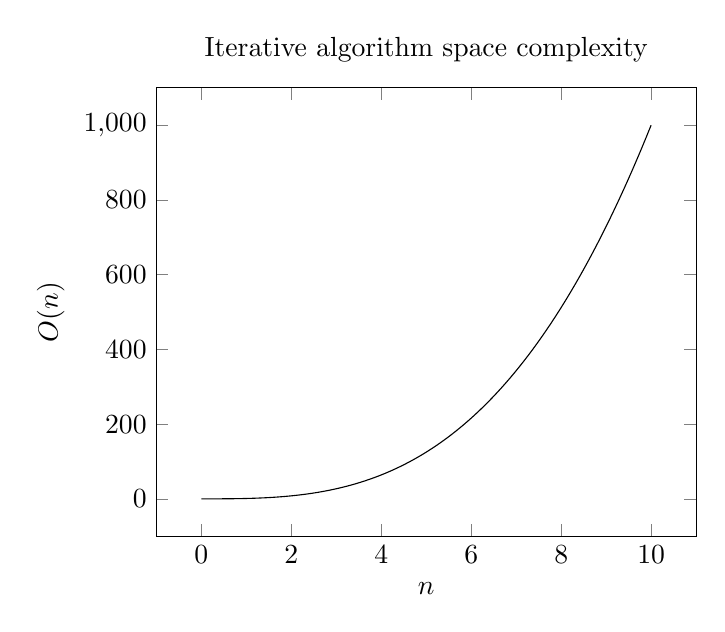
\begin{tikzpicture}
    \begin{axis}[
        title={Iterative algorithm space complexity},
        xlabel=$n$,
        ylabel={$O(n)$}
    ]
    \addplot [
        domain = 0:10,
        samples = 100
        ]{x^3};
    \end{axis}
\end{tikzpicture}

Perkalian matriks merupakan perkalian antara 2 buah matriks persegi yang mempunyai ukuran yang sama untuk menghasilkan sebuah matriks baru. Perkalian matriks dengan ukuran yang kecil sangat mudah dilakukan dengan perhitungan manual, namun akan sangat sulit apabila matriks memiliki ukuran yang besar. Untuk memudahkan perkalian matriks yang berukuran besar, maka dapat dilakukan perkalian dengan bantuan program yang dikembangkan dari pemrograman bahasa C. 

Ada beberapa algoritma yang dapat digunakan dalam menghitung perkalian matriks diantaranya yaitu algortima strassen, iterative, dan rekursif. Algoritma tersebut tentunya memiliki karakteristik yang berbeda-beda. Algoritma yang baik adalah algoritma yang memiliki efisiensi yang baik ketika digunakan untuk menghitung data yang besar. Dalam percobaan ini kita akan membandingkan tingkat efisiensi dari masing-masing algoritma. 

Algoritma yang baik adalah algoritma yang mangkus atau efisien. Untuk menentukan tingkat kemangkusan algoritma, diperlukan metode yang dapat digunakan sebagai dasar analisa. Selain itu juga diperlukan parameter khusus yang dapat dijadikan tolak ukur agar algoritma dapat dikatakan mangkus. 

Tujuan dari percobaan ini adalah menentukan tingkat kemangkusan dari masing-masing algoritma sehingga dapat diketahui algoritma yang terbaik untuk melakukan perkalian matrikas dengan ukuran yang besar.

Metode analisa yang digunakan dalam percobaan ini adalah analisa kompleksitas waktu dan ruang. Ada 4 algoritma yang di analisa yaitu algortima strassen, iterative, rekursif, dan divide and conquer.

\section{Studi Pustaka}

\subsection{Bahasa Pemrograman C}

Bahasa pemrograman adalah suatu bahasa yang hanya dapat dimengerti oleh komputer.
 Komputer tidak akan jalan tanpa perintah dari kita. Dengan perintah yang kita 
 berikan kepada komputer tersebut, maka komputer tersebut akan membacanya dan 
 memberikan output yang kita inginkan. Banyak bahasa pemrograman yang kita akan 
 temui dan pelajari (sebut saja bahasa C, Cplus-plus, Java, dan lain-lainnya) pada 
 saat kita ingin membuat suatu program. Namun, untuk artikel ini, kita akan berfokus
  terhadap bahasa yang sering kalian temui sebagai pemula, yaitu bahasa C.
Bahasa C adalah bahasa pemrograman prosedural yang dapat digunakan untuk 
membangun software seperti operating system, database, dan lainnya. Bahasa ini 
diciptakan oleh Dennis Ritchie untuk menciptakan aplikasi sistem yang dapat berinteraksi 
dengan hardware secara langsung. Bahasa ini juga mempunyai beberapa fakta yang menarik 
seperti menjadi penerus bahasa B, menjadi bahasa yang menciptakan operating system yang
 bernama UNIX, dan telah diformalkan oleh American National Standard Institute (ANSI) pada tahun 1988.
Bahasa C tentunya adalah bahasa yang dapat dijadikan sebagai bahasa pemrograman
 pertama bagi pemula. Namun, perlu kalian ketahui bahwa bahasa C juga dikenal sebagai 
 mother language, system programming language, procedure-oriented programming language, 
 structured programming language, dan mid-level programming language. Berikut penjelasannya.
Bahasa C dikenal sebagai mother language karena sebagian besar compiler, kernel,
 dan lainnya dicatat dalam bahasa ini dan beberapa bahasa pemrograman lainnya 
 mengikuti syntax bahasa ini seperti C++, Java, dan lainnya. Bahasa C sebagai system 
 programming language dapat digunakan untuk melakukan low-level programming. 
 Bahasa C sebagai procedural language menentukan beberapa langkah untuk program 
 agar dapat menyelesaikan masalah. Bahasa C sebagai structured procedural language 
 berarti bahasa ini dapat memecahkan sebuah program menjadi bagian-bagian sehingga
  dapat dimengerti dengan mudah. Bahasa C sebagai mid-level programming language 
  mendukung kedua low-level dan high-level language.
Tentunya, bahasa C dapat digunakan untuk kehidupan sehari-hari kita karena 
bahasa ini menghasilkan kode yang berjalan hampir secepat kode yang ditulis dalam assembly language. Contoh penggunaan bahasa C antara lain Operating Systems, Language Compilers, Text Editors, Network Drivers, Databases, dan Utilities.

\subsection{Matriks}
Matriks adalah kumpulan bilangan yang disusun secara baris atau kolom atau kedua-duanya dan di dalam suatu tanda kurung. Bilangan-bilangan yang membentuk suatu matriks disebut sebagai elemen-elemen matriks. Matriks digunakan untuk menyederhanakan penyampaian data, sehingga mudah untuk diolah.

\subsubsection{ukuran matriks}
Ukuran matriks ditentukan oleh jumlah baris dan kolom yang dikandungnya. Matriks dengan kolom m dan n baris disebut matriks m x n atau matriks "m kali n", dimana m dan n disebut dimensinya. Sebagai contoh, matriks A di bawah adalah matriks 3 x 2. Matriks dengan satu baris disebut vektor baris, dan matriks dengan satu kolom disebut vektor kolom. Matriks dengan jumlah baris dan kolom yang sama disebut matriks persegi. Matriks dengan jumlah baris atau kolom yang tak terbatas (atau keduanya) disebut matriks tak terbatas. Dalam beberapa konteks, akan bermanfaat untuk mempertimbangkan sebuah matriks tanpa baris atau tanpa kolom, yang disebut matriks kosong.

\begin{figure}[htbp]
    \includegraphics[width=5cm]{gambar/contoh.jpg}
    \centering
    \caption{matriks 3x2}   
\end{figure}

\subsubsection{Perkalian Matriks}
Perkalian dua matriks ini bisa dilakukan ketika jumlah kolom A dan jumlah baris B sama. Perkalian matriks tersebut akan menghasilkan suatu matriks dengan jumlah baris yang sama antara matriks A dan B. Syarat dua buah matriks bisa dikalikan jika mempunyai jumlah kolom matriks pertama sama dengan jumlah baris matriks ke dua. Adapun ordo matriks hasil perkalian dua matriks adalah jumlah baris pertama dikali jumlah kolom ke dua.
Misalnya matriks P memiliki jumlah kolom sebanyak a dan jumlah baris c. Sedangkan matriks Q memiliki jumlah kolom sebanyak c dan jumlah baris a. Hasil perkalian P dan Q adalah matriks R dengan jumlah kolom a dan jumlah baris d.
Perkalian dua buah matriks dapat dilihat pada contoh di bawah ini:
\begin{figure}[htbp]
    \includegraphics[width=5cm]{tabel_matriks.jpg}
    \centering
    \caption{deskripsi ukuran matriks}        
\end{figure}


\section{Metodologi Penelitian}
Penelitian dilakukan dengan membuat program perkalian dengan dimensi matriks 
yang kecil yaitu ukuran 3x3. Selanjutnya dilakukan perhitungan manual perkalian
 matriks ukuran 3x3. Dimasukkan dengan angka yang sama antara perhitungan program
  dan perhitungan manual. Selanjutnya diamati hasil dari kedua perhitungan
   tersebut. Setelah hasil benar, kemudian dikembangkan perhitungan untuk 
   ukuran 10x10, 100x100, dan 1000x1000.

\begin{center}
    \tikzset{priority arrow/.append style={rotate=180,anchor=0,xshift=30}}
    \smartdiagram[priority descriptive diagram]{Jika valid, program dikembangkan untuk ukuran besar,Pengamatan kedua hasil,Perhitungan manual,Pembuatan program}
\end{center}

\section{Pembahasan}

\subsection{Flowchart algoritma program}
program memiliki flowchart sebagai berikut:

\begin{figure}[htbp]
    \includegraphics[width=5cm]{flowchart.jpg}
    \centering
    \caption{flowchart program perkalian matriks}        
\end{figure}


\subsection{Perhitungan Kompleksitas waktu}


\section{Kesimpulan}
Program berjalan dengan baik ketika dimensi atau ordo matriks berada dibawah ordo 50x50. Saat berada pada ordo diatas 50x50 perhitungan program berjalan akan tetapi tidak dapat menampilkan hasil secara keseluruhan. Kemudian pada ordo diatas 1000x1000 program tidak dapat berjalan.

% Referensi
\begin{thebibliography}{00}
    \bibitem{b1} K. H. Rosen, Discrete Mathematics and It’s Applications - Seventh
    Edition. McGraw-Hill.Inc, 2012.
    \bibitem{b2} Solichin, Achmad, Pemrograman Bahasa C dengan Turbo C, 2003.
    \end{thebibliography}

\end{document}